\documentclass[11pt]{gsasthesis} % 10,11 and 12pt fonts allowed

%%%%%%%%%%%%%%%% PACKAGES YOU PROBABLY WANT %%%%%%%%%%%%%%%%
% Include packages you want. The gsasthesis style file already includes
% packages "setspace" and "tocbibind".

\usepackage{etex} % extend the number of registers

% GSAS: "all margins should be at least 1 inch."
\usepackage[margin={1.2in}]{geometry}
% If you want asymmetric margins for two-sided documents, use the "twoside"
% option, as in
% \usepackage[top=1in,bottom=1.5in,left=1in,right=1.5in,twoside]{geometry} The
% left and right options become inner and outer margins The default horizontal
% latex margin ratio is 2:3. The default vertical top:bottom margin ratio is 2:3
% also. You can also set it directly by passing the hmarginratio option to the
% geometry package, as in
% \usepackage[top=1in,left=1in,vmarginratio=2:3,hmarginratio=2:5,twoside]{geometry}

% Appendix package. Not necessary, but it does make managing appendices easier
\usepackage[titletoc]{appendix}

%%%%%%%%%%%%%%%% PACKAGES MAY WANT %%%%%%%%%%%%%%%%

% sideways tables and figures
\usepackage{rotating}

% tables that spill over multiple pages
\usepackage{longtable}

% references
%\usepackage{natbib}

\usepackage{comment}

\usepackage{multirow, booktabs}
\usepackage{amsmath}
\usepackage{amssymb}
\usepackage{amsfonts}
\usepackage{makecell}

\usepackage{enumitem}

\usepackage{graphicx}
\usepackage{soul}
\usepackage[normalem]{ulem}
\usepackage{subcaption}

\newcolumntype{L}[1]{>{\raggedright\let\newline\\\arraybackslash\hspace{0pt}}m{#1}}
\newcolumntype{C}[1]{>{\raggedright\let\newline\\\arraybackslash\hspace{0pt}}m{#1}}

\usepackage{CJKutf8}
\usepackage{pifont}
\newcommand{\xmark}{\ding{55}}

\usepackage{rotating}
\usepackage{pdflscape}

% fonts that are nicer than defaults
\usepackage[sc]{mathpazo}
\usepackage{courier}

% Use 8-bit encoding that has 256 glyphs, pretty please
\usepackage[utf8]{inputenc}
\usepackage[T1]{fontenc}

% babel is required for blindtext, which generates random text
\usepackage[english]{babel}
\usepackage{blindtext}

% math support
\usepackage{amsmath}

% Slightly tweak font spacing for aesthetics
\usepackage{microtype}



% You need the footmisc package with the stable option if you want to have
% footnotes inside section titles, for example to say that a particular chapter
% has been co-authored with someone. The multiple option ensures that there is a
% comma between two consecutive footnotes
\usepackage[stable,multiple]{footmisc}


% Nicer captions
\RequirePackage[font=small,format=plain,labelfont=bf,textfont=it]{caption}
\addtolength{\abovecaptionskip}{1ex}
\addtolength{\belowcaptionskip}{1ex}


%%%%%%%%%%%%%%%% COMPULSORY FIELDS %%%%%%%%%%%%%%%%

\title{Title of Your Ph.D. Thesis} % needs to match title on DAC
\author{Your Name} % full name as it appears on your GSAS record, needs
                          % to match name on DAC
\degreename{Doctor of Philosophy}
\degreefield{Systems Engineering and Engineering Management} % Official name of subject as listed in GSAS
                                % handbook
\department{Systems Engineering and Engineering Management} % official name of department
\degreemonth{January} % Month of Defense (i.e. month when DAC was signed)
\degreeyear{2021} % Year the DAC was signed
\principaladvisor{Professor AA}

% Optionally, you can add a second advisor, but you can't have three
%\secondadvisor{Professor George Secondary}



\begin{document}

%%%%%%%%%%%%%%%% FRONTMATTER %%%%%%%%%%%%%%%%

\pagenumbering{roman} % GSAS wants roman page numbers for frontmatter

% the following four pages are required in that order. The first two pages are
% not allowed to have page numbers, this is taken care of in the class file.
\thesistitlepage
%\copyrightpage
\committeepage
\begin{abstract}
\end{abstract}

\begin{cabstract}


\end{cabstract}

% Center headings for table of contents, LOT, and LOF and make them smaller so
% that "Abstract", "Acknowledgments" and "Contents" all look alike. Comment out
% if you want the default. If you want more control, use the "tocloft" package.
\renewcommand{\contentsname}{\protect\centering\protect\Large Contents}
\renewcommand{\listtablename}{\protect\centering\protect\Large List of Tables}
\renewcommand{\listfigurename}{\protect\centering\protect\Large List of Figures}

\tableofcontents % Table of contents

% The rest of the front matter: Lists of tables, figures, dedication and
% acknowledment is optional. Comment out whatever you don't like
\listoftables
\listoffigures
\begin{acknowledgments}
  Acknowledgement here.   
  
  %I would like to thank my thesis committee members for their valuable and constructive comments. Furthermore, I want to express my gratitude to the professors in the Department of Systems Engineering and Engineering Management.  
\end{acknowledgments}
%\begin{dedication}
%  To my parents and my girl friend. 
%\end{dedication}


%%%%%%%%%%%%%%%% MAIN BODY %%%%%%%%%%%%%%%%
\pagenumbering{arabic} % reset page numbering and switch to arabic

% Introductory chapter. Comment out if you don't have an intro chapter, but I
% think most committees expect you to have one.
% Don't number the intro chapter, but add to to the table of contents
%\addcontentsline{toc}{chapter}{Introduction}
\chapter{Introduction}\label{ch:intro}
Introduction, motivation and big picture of your phd thesis

\section{Contributions}
The contributions of this dissertation are summarized as follows:
\begin{itemize}[leftmargin=*]
    \item \textbf{Description of your first paper}\\
    \item \textbf{Description of your second paper}\\
    \item $\cdots$
\end{itemize}


\section{Produced Publications}
The research work of this dissertation has produced some direct and indirect publications as listed below:
%\noindent \bullet xx \\
\begin{itemize}
    \item $\cdots$
\end{itemize}


\section{Thesis Outline}



\chapter{Literature Review}\label{ch:background}
\section{Unsupervised Language Model Pre-training}
The advent of unsupervised Language Model (LM) pre-training has led to significant performance gains on a variety of language understanding~\citep{radford2018improving,devlin-etal-2019-bert,yang2019xlnet,clark2020electra} and language generation~\citep{radford2019language,dong2019unified} tasks. Typically, a deep Long Shot-Term Memory networks (LSTM)~\citep{hochreiter1997long,peters-etal-2018-deep} or Transformer~\citep{vaswani2017attention} is first pre-trained on large-scale corpus and then the contextualized embeddings from the pre-trained language model are provided for the downstream tasks in the manner of feature extraction or fine-tuning.


\begin{sidewaysfigure}
    \centering
    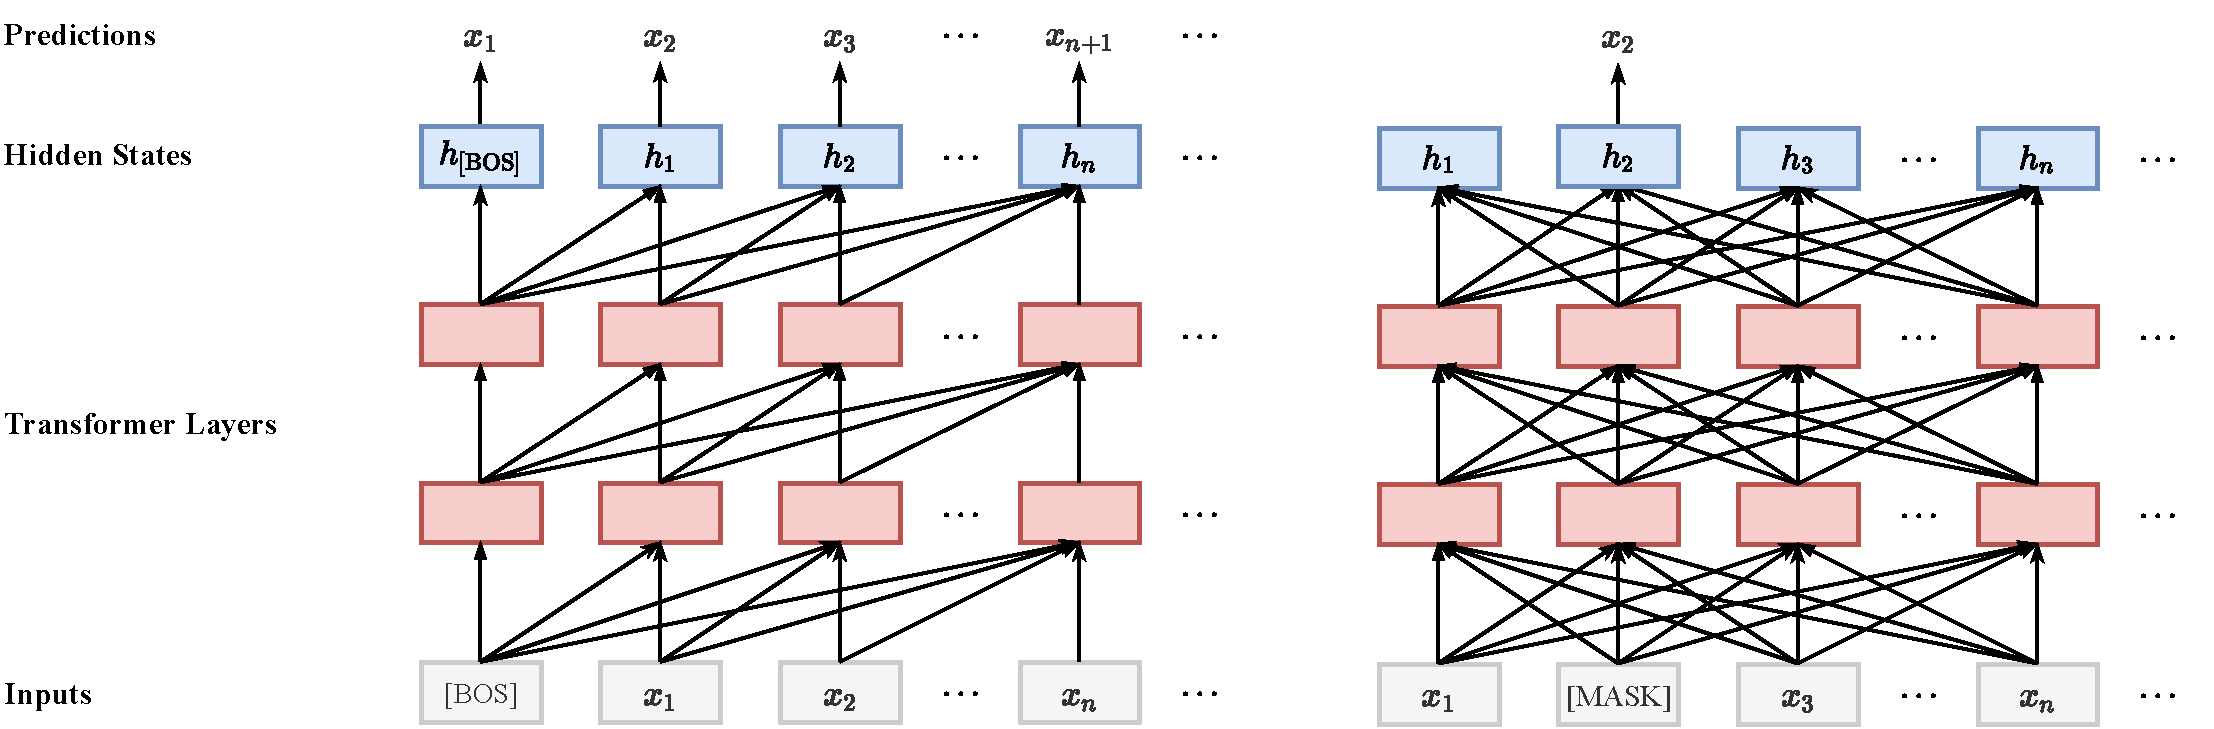
\includegraphics[width=\textwidth]{fig/ptlm.pdf}
    \caption{Auto-regressive language modeling (left) and masked language modeling (right).}
    \label{fig:ptlm}
\end{sidewaysfigure}

Several pre-training techniques have been developed for generating general-purpose contextualized embeddings. \citet{peters-etal-2017-semi,peters-etal-2018-deep} employ two unidirectional LSTM LMs, namely, a forward left-to-right LM and a backward right-to-left LM, to encode bi-directional contexts and the pre-training is conducted via auto-regressive language modeling, as shown in the left part of Figure~\ref{fig:ptlm}. GPT~\citep{radford2018improving} and GPT-2~\citep{radford2019language} adopt the same auto-regressive pre-training objective but change to model sequential word flow with unidirectional Transformer. BERT~\citep{devlin-etal-2019-bert}, as well as its variants~\citep{conneau2019cross,liu2019roberta,wang2019structbert,joshi-etal-2020-spanbert}, propose to learn contextualized embeddings based on masked language modeling---reconstruct the masked input with the special \texttt{[MASK]} token and the surrounding context (see the right part of Figure~\ref{fig:ptlm}). In order to unify the auto-regressive pre-training and auto-encoding based pre-training, UniLM~\citep{dong2019unified} jointly optimizes the pre-training of Transformer with auto-regressive language modeling objective and masked language modeling objective. Similarly, XLNet~\citep{yang2019xlnet} designs permutation language modeling objective to capture the context information from all positions while preserving the temporal dependency among the predictions. MASS~\citep{song2019mass}, BART~\citep{lewis-etal-2020-bart} and T5~\citep{raffel2019exploring} are the initial attempts to pre-train sequence-to-sequence architecture and achieve promising results on machine translation and abstractive summarization. 


\section{Multilingual Language Model Pre-Training}
Multilingual language model pre-training is a multilingual extension of language model pre-training, where the deep neural architecture~\citep{vaswani2017attention,peters-etal-2018-deep} is pre-trained on large-scale multilingual corpus, e.g., a collection of wikipedia documents in different languages. The yielding multilingual pre-trained language models (mPTLMs)~\citep{che-etal-2018-towards,devlin-etal-2019-bert,conneau2019cross,mulcaire-etal-2019-polyglot,conneau-etal-2020-unsupervised} have been regarded as the gold standard for a variety of unsupervised cross-lingual natural language understanding tasks~\citep{prettenhofer-stein-2010-cross,schwenk-li-2018-corpus,zeman-etal-2018-conll,liu-etal-2019-xqa}. The most impressive features of mPTLMs is that even performing cross-lingual transfer in a zero-shot manner---only fine-tune the mPTLMs on the source-language training data---it can still significantly outperform the existing works based on cross-lingual embeddings~\citep{mikolov2013exploiting,faruqui-dyer-2014-improving,smith2018offline} or machine translation~\citep{banea-etal-2008-multilingual,duh-etal-2011-machine}, as observed in~\citet{pires-etal-2019-multilingual,wu-dredze-2019-beto,keung-etal-2019-adversarial,artetxe-etal-2020-cross}. After being additionally trained on machine-translated data from source language, the cross-lingual performances of the cross-lingual models exploiting mPTLMs are further improved~\citep{huang-etal-2019-unicoder,conneau-etal-2020-unsupervised,cao2020multilingual}, especially on sequence classification~\citep{schwenk-li-2018-corpus} and sequence pair classification tasks~\citep{conneau-etal-2018-xnli,yang-etal-2019-paws}.


\chapter{Chapter 3}\label{ch:ate}

\chapter{Chapter 4}

\chapter{Chapter 5}

\chapter{...}



%%%%%%%%%%%%%%%% BACK MATTER %%%%%%%%%%%%%%%%

% Put appendices, bibliography, and supplemental materials here

% The bibliography may be single spaced within each entry, but must be
% double-spaced between each entry. Most bibliography styles leave space between
% entries, so that shouldn't be a problem.
\begin{singlespacing}
  % I like "References" better than "Bibliography"
  \renewcommand{\bibname}{References}

  % Any bibliohgraphy style that leaves space between entries is fine
  \bibliographystyle{acl_natbib}
  %\bibliographystyle{ecca}
  \bibliography{references}
\end{singlespacing}

% Appendices from all chapters should go at the end
%\input{appendix}

\end{document}
